\setchaptergraphic{
    % Cauchy sequence convergence
    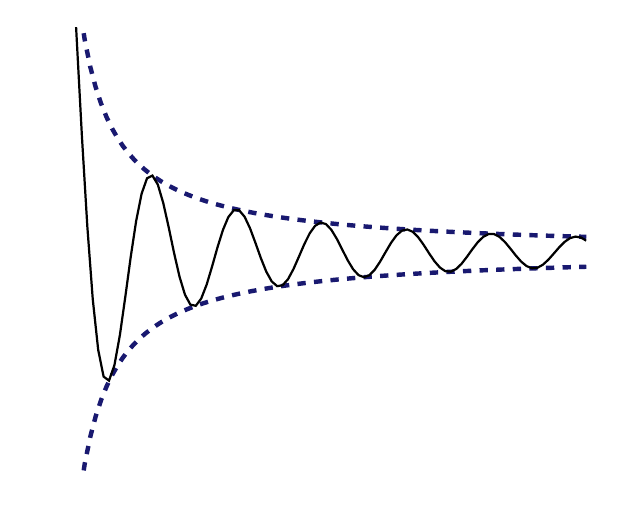
\begin{tikzpicture}[scale=1.0]
        \begin{axis}[
            xmin=0,xmax=20,
            ymin=-0.75,ymax=0.75,
            axis line style={draw=none},
            tick style={draw=none},
            xticklabels=\empty,
            yticklabels=\empty,
        ]
            \addplot[domain=0:20, MidnightBlue, dashed, ultra thick, samples=100] {+1/x};
            \addplot[domain=0:20, MidnightBlue, dashed, ultra thick, samples=100] {-1/x};
            \addplot[domain=0.1:20, black, thick, samples=100] {sin(deg(2*x))/x};
        \end{axis}
    \end{tikzpicture}
}

\chapter{Analysis}
\label{ch:analysis}

\section{Fields}

\begin{defn}
    A \emph{field} $(F, +, \cdot)$ is a set $F$ equipped with two binary operations called addition ($+$) and multiplication ($\cdot$), which do not necessarily correspond to addition and multiplication on the real numbers.

    Field axioms:
    \begin{itemize}
        \item Addition and multiplication are commutative.
        \item Addition and multiplication are associative.
        \item Additive and multiplicative identities, denoted $0$ and $1$ respectively.
        \item Every element $x \in F$ has an additive inverse denoted $-x$.
        \item Every element $x \in F$ where $x \neq 0$ has a multiplicative inverse denoted $x^{-1}$ or $1/x$.
        \item Multiplication is distributive over addition.
    \end{itemize}
\end{defn}

\begin{thm}{Field properties}\label{field-properties}\proofbreak
    For every $x, y, z \in F$:
    \begin{enumerate}
        \item $0 \cdot x = 0$
        \item $(-1) \cdot x = -x$
        \item $-(-x) = x$
        \item If $x \neq 0$, $\left(x^{-1}\right)^{-1} = x$
        \item $x \cdot (-y) = -(x\cdot y)$
        \item $(xy)^{-1} = x^{-1}y^{-1}$
        \item $x\cdot(y-z) = x\cdot y - x \cdot z$
        \item $-(x - y) = y - x$
    \end{enumerate}
\end{thm}

\begin{proof}\proofbreak
    \begin{enumerate}
        \item $0 \cdot x + 0 \cdot x = (0 + 0) \cdot x = 0 \cdot x$. Since the additive identity is unique, this implies that $0 \cdot x = 0$.
        \item $(-1) \cdot x + x = (-1) \cdot x + 1 \cdot x = (-1 + 1) \cdot x = 0 \cdot x = 0$. Therefore, $(-1) \cdot x = -x$.
        \item Let $w = -x$, then $x + w = 0$. Therefore, $x = -w$, and so $x = -(-x)$.
        \item Let $w = x^{-1}$, then $wx = 1 = xw$, so $x = w^{-1}$. Therefore, $x = w^{-1}$, and so $(x^{-1})^{-1} = w^{-1} = w$.
        \item $x \cdot (-y) + xy = x\cdot(-y + y) = x\cdot 0 = 0$.
        \item Let $(xy)(x^{-1}y^{-1}) = (yx)(x^{-1}y^{-1}) = y(xx^{-1})y^{-1} = yy^{-1} = 1$. Since the multiplicative identity is unique, $(xy)^{-1} = x^{-1}y^{-1}$.
        \item $x \cdot (y-z) = x \cdot (y + (-1)z) = x\cdot y + x \cdot (-1)z = xy - xz$.
        \item Since $(x - y) + (y-x) = x + (-y + y) - x = x - x = 0$, we know $-(x - y) = (y - x)$.
    \end{enumerate}
\end{proof}

\begin{defn}
    Let $F$ be a field, and let $x \in F$ and $n \in Z$, $n \geq 0$. Then we recursively define
    \[x^n =
        \begin{dcases}
            1, & n = 0 \\
            x \cdot x^{n-1}, & n > 0
        \end{dcases}.
    \]
\end{defn}

\begin{defn}
    An \emph{ordered field} is a field $(F, +, \cdot)$ together with a subset $F^+ \subset F$ such that\begin{itemize}
        \item For all $x, y \in F^+$, both $x + y$ and $x \cdot y$ are in $F^+$.
        \item (Trichotomy) For all $x \in F$, exactly one of $x \in F^+$, $-x \in F^+$, or $x = 0$ is true.
    \end{itemize}
\end{defn}

If $(F, F^+)$ is an ordered field and $x \in F$, we say $x$ is positive (or $x > 0$) if $x \in F+$.

\begin{defn}
    For elements $x, y$ in an ordered field, we say $x > y$ (or $y < x$) if $x - y > 0$, and $x \geq y$ (or $y \leq x$) if $x = y \lor x > y$.
\end{defn}

\begin{thm} For all $x, y, z, w \in F$, where $F$ is an ordered field:
    \begin{enumerate}
        \item $(x < y) \land (y < z) \implies (x < z)$.
        \item $(x < y) \land (z < w) \implies x + z < y + w$.
        \item $(x > 0) \land (y < 0) \implies xy < 0$.
        \item $(x < 0) \land (y < 0) \implies xy > 0$.
        \item $x \neq 0 \implies x^2 > 0$.
    \end{enumerate}
\end{thm}

\begin{proof}\proofbreak
    \begin{enumerate}
        \item $x < y \land y < z$ implies that $y - x > 0$ and $z - y > 0$. Therefore, $(y - x) + (z - y) = z - x > 0$, so $x < z$.
        \item $x < y \land z < w$ implies that $y - x > 0$ and $w - z > 0$. Therefore, $(y - x) + (w - z) = (y + w) - (x + z) > 0$, so $x + z < y + w$.
        \item $(x > 0) \land (y < 0)$ implies that $-y > 0$. Since $x(-y) > 0$ and $x(-y) = -(xy)$, it follows that $xy < 0$.
        \item $(x < 0) \land (y < 0)$ implies that $(-x)(-y) > 0$. Since $(-x)(-y) = -(-xy) = -(-xy) + (xy  + (-xy)) = (-xy) - (-xy) + xy = 0 + xy = xy$, it follows that $xy > 0$.
        \item If $x > 0$, then $x^2 > 0$. If $x < 0$, then $-x > 0$, so $(-x)^2 > 0$. Since $(-x)(-x) = x^2$, it follows that $x^2 > 0$.
    \end{enumerate}
\end{proof}

\begin{prop}\label{trichotomy-exclusion}
    Let $(F, F^+)$ be an ordered field, and $x, y \in F$. Then at most one of the following is true: $x < y$, $x > y$.
\end{prop}

\begin{proof}
    For the sake of contradiction, assume that $x < y$ and $y > x$. Since $x < y$, we know $y - x > 0$, so $(y - x) \in F^+$. Since $x > y$, we know that $y - x < 0$, so $(y - x) \in F^-$. This contradicts trichotomy, $x < y \land y > x$ cannot be true.
\end{proof}

\begin{prop}\label{greater-than-ratio}
    Let $(F, F^+)$ be an ordered field, and let $x, y \in F^{+}$. Then $x > y$ if and only if $\frac{x}{y} > 1$.
\end{prop}

\begin{proof}\proofbreak
    ($\implies$) If $x > y$, by definition $x - y > 0$. Therefore, $\frac{x}{y} - \frac{y}{y} > 0$, so $\frac{x}{y} - 1 > 0$. This implies that $\frac{x}{y} > 1$.

    ($\impliedby$) If $\frac{x}{y} > 1$, we know that $\frac{x}{y} - 1 > 0$, so it follows that $x - y > 0$. Therefore, we have $x > y$.
\end{proof}

\begin{prop}\label{average-in-between}
    Let $F$ be an ordered field, and $x, y \in F$ with $x < y$. Then $x < \frac{x+y}{2} < y$.
\end{prop}

\begin{proof}
    Since $x < y$, we know that $x + x < x + y$, so $(x + y) - 2x > 0$. Then $\frac{x+y}{2} - x > 0$, so $x < \frac{x+y}{2}$. Similarly, since $x < y$ we know that $x + y < y + y$, so $2y - (x + y) > 0$. Then we have $y - \frac{x + y}{2} > 0$, so $\frac{x + y}{2} < y$. Therefore, $x < \frac{x+y}{2} < y$.
\end{proof}

\begin{prop}\label{multiplicative-inequality-one}
    Let $F$ be an ordered field, and let $a, b, x \in F^+$ such that $a < b$. Then $ax < bx$.
\end{prop}

\begin{proof}
    Since $a < b$, by definition $b - a > 0$. Since $x > 0$, it follows that $x(b-a) > 0$, and so $xb - xa > 0$. Therefore, $ax < bx$ by definition.
\end{proof}

\begin{prop}\label{multiplicative-inequality-two}
    Let $F$ be an ordered field, and let $a, b, c, d \in F^+$ such that $a < b$ and $c < d$. Then $ac < bd$.
\end{prop}

\begin{proof}
    By Proposition \ref{multiplicative-inequality-one}, we know that $ac < bc$, and similarly that $bc < bd$. It follows by transitivity that $ac < bd$.
\end{proof}

\begin{prop}\label{square-is-positive-or-zero}
    Let $F$ be an ordered field, and $x \in F$. Then $x^2 \geq 0$, and $x^2 = 0$ if and only if $x = 0$.
\end{prop}

\begin{proof}
    If
    \begin{itemize}
        \item $x = 0$, then $x^2 = 0(0) = 0$,
        \item $x > 0$, then $x^2 \in F^+$, and so $x^2 > 0$,
        \item $x < 0$, then $(-x)^2 \in F^+$, and since $(-x)^2 = (-1)^2x^2 = x^2$, it follows that $x^2 > 0$.
    \end{itemize}
\end{proof}

\section{Bounds}

\begin{defn}
    Let $S$ be an ordered set, and $E \subseteq S$. An \emph{upper bound} of $E$ in $S$ is $\beta \in S$ such that $\alpha \leq \beta$ for all $\alpha \in E$.
\end{defn}

\begin{defn}
    An upper bound $\beta$ of $E$ in $S$ is a \emph{least upper bound} when $\alpha < \beta$ implies $\alpha$ is not an upper bound for $E$, for all $\alpha \in S$.
\end{defn}

\begin{defn}
    An ordered set $S$ has the \emph{least upper bound property} if every $E \subseteq S$ has a least upper bound. We also say that $S$ is \emph{complete}.
\end{defn}

\begin{prop}
    Let $S$ be an ordered set, and $A$ and $B$ be bounded subsets of $S$. Then $\sup (A \union B) = \max (\sup A, \sup B)$.
\end{prop}

\begin{prop}
    Define $A + B = \left\{x + y \compbar x \in A, y \in B\right\}$. Then $\sup A + B = \sup A + \sup B$.
\end{prop}

\begin{proof}
    For any $p \in A + B$, $p = a + b$ for some $a \in A$ and $b \in B$. Since $a \leq \sup A$ and $b \leq \sup B$, it follows that $p \leq \sup A + \sup B$. Suppose $\sup A + \sup B > \sup A + B$, then since $a + b \leq \sup (A + B)$, it follows $a \leq \sup (A + B) - b$ for any $a \in A$ and $b \in B$. Then $b \leq \sup (A + B) - \sup A$ and so $\sup B \leq \sup (A + B) - \sup A$ for any $a \in A$ and $b \in B$. Therefore, $\sup A + \sup B \leq \sup (A + B)$.
\end{proof}

\begin{prop}
    If $A \leq B$ then $\sup A \leq \sup B$.
\end{prop}

\begin{proof}
    Since $b \leq \sup B$ for all $b \in B$, it follows that $a \leq \sup B$ for all $a \in A$ and so $\sup A \leq \sup B$.
\end{proof}

\section{Real Numbers}

\begin{defn}
    A \emph{sequence} in a set $X$ is a function $f: \Z_{\geq k} \to X$.
\end{defn}

\begin{exmp}
    Let $f: \Z_{\geq 3} \to Q$ be the function given by $f(n) = \frac{(-1)^n}{n}$.
\end{exmp}

\begin{defn}
    Let $F$ be an ordered field, and $f$ a sequence in $F$. Then we say that $f$ \emph{converges} to some \emph{limit} $x \in F$ if, for every open interval $(a, b) \in F$ containing $x$, there exists $N \in Z_{\geq k}$ such that $f(n) \subseteq (a, b)$ for every $n \geq N$.
\end{defn}

\begin{thm}
    If a sequence $f$ in an ordered field $F$ is convergent, it has a unique limit.
\end{thm}

\begin{proof}
    Assume that a convergent sequence $f$ converges to two distinct limits, $L_1, L_2 \in F$. Since $L_1 \neq L_2$, one must be greater than the other, so without loss of generality we will assume that $L_1 < L_2$. By Proposition \ref{average-in-between}, we know that $L_1 < \frac{L_1+L_2}{2} < L_2$. Construct the open intervals $I_1 = (L_1 - 1, \frac{L_1+L_2}{2})$ and $I_1 = (\frac{L_1+L_2}{2}, I_2 + 1)$. Since $f$ converges to both $L_1$ and $L_2$, there must exist some $N_1, N_2 \in \Z$ such that for all $n \geq N_1$ we have $f(n) \in I_1$, and for all $n \geq N_2$ we have $f(n) \in I_2$. Now let $N$ be the largest of $N_1$ and $N_2$. For any $n \geq N$, we have $f(n) \in I_1$ so $f(n) < \frac{L_1+L_2}{2}$, and for any $n \geq N$, we have $f(n) \in I_2$ so $f(n) > \frac{L_1+L_2}{2}$. By Proposition \ref{trichotomy-exclusion}, this is a contradiction, so it must be that $f$ has a distinct limit.
\end{proof}

\begin{defn}
    A \emph{binary search sequence} in an ordered field $F$ is $\left\{[a_n, b_n]\right\}_{n \geq k}$ with $a_n, b_ \in F$ satisfying $[a_{n+1}, b_{n+1}] \subseteq [a_n, b_n]$ and $b_{n+1}-a_{n+1} = \frac{1}{2}(b_n - a_n)$.
\end{defn}

\begin{defn}
    A binary search sequence \emph{converges} to some $x \in F$ if for all $n \geq k$, $\left\{[a_n, b_n]\right\}$ contains $x$.
\end{defn}

\begin{defn}
    An ordered field $F$ is \emph{complete} if every binary search sequence converges to a unique element of $F$.
\end{defn}

\begin{defn}
    Any complete ordered field is a model for the real numbers.
\end{defn}

\begin{rmk}
    Any two complete ordered fields are isomorphic.
\end{rmk}

\begin{thm}\label{archimedean-property}
    The Archimedean property states that for any $x, y \in \R^{+}$, there exists $n \in \Z_{\geq 1}$ such that $nx > y$.
\end{thm}

\begin{proof}
    For the sake of contradiction, assume there exists some $x, y \in \R^{+}$ such that there is no $n \in \Z$ such that $nx > y$. Therefore, there is some $z \in \R$ where $z = y/x$ such that $z \geq n$ for all $n \in \Z$. Since $2^k \in \Z$ for all $k \in \Z$, it follows that $\frac{z}{2^k} \geq 1$ by Proposition \ref{greater-than-ratio}.

    Now consider the binary search sequence $f(k) = \left\{[0, \frac{z}{2^k}]\right\}_{k \geq 0}$. It is clear that $0 \in f(k)$ for all $k \in \Z_{\geq 0}$, however since $\frac{z}{2^k} \geq 1$, we also have that the $1 \in f(k)$ for all $k \in \Z_{\geq 0}$. This would imply that the binary search sequence converges to both $0$ and $1$, which contradicts the definition of the real numbers, so it follows that there is no such $z \in \R$.
\end{proof}

\begin{cor}
    Suppose $x \in \R$ satisfies $0 \leq x \leq \frac{1}{n}$ for every $n \in \Z_{\geq 1}$. Then $x$ must be zero.
\end{cor}

\begin{proof}
    Assume, for the sake of contradiction, that $x \neq 0$. Then by the Archimedean property \ref{archimedean-property}, there exists $n \in \Z_{\geq 1}$ such that $nx > 1$, and so $x > \frac{1}{n}$ by Proposition \ref{greater-than-ratio}. This is a contradiction, and so $x = 0$.
\end{proof}

\begin{thm}\label{bernoullis-inequality}Bernoulli's inequality\proofbreak
    Let $n \in \Z$, $x \in \R$ such that $n \geq 0$ and $x \geq -1$. Then \[(1 + x)^n \geq 1 + nx.\]
\end{thm}

\begin{proof}
    We will proceed by induction on $n$. For $n=0$, we have $(1 + x)^0 = 1$, and $1 + 0x = 1$, and so the base case is true since $1 \geq 1$.

    Assume that $(1 + x)^n \geq 1 + nx$ for some $n \geq 0$. Then
    \begin{align*}
        (1 + x)^{n+1} &= (1 + x)(1 + x)^n \\
        &= (1 + x)^n + x(1 + x)^n.
    \end{align*}
    Since $(1 + x)^n \geq 1 + nx$, we then have
    \begin{align*}
        (1 + x)^{n+1} &= (1 + x)^n + x(1 + x)^n \\
        &\geq 1 + nx + x(1 + nx) \\
        &= 1 + (n+1)x + nx^2
    \end{align*}
    Note that $x^2 \in \R^+$ by Proposition \ref{square-is-positive-or-zero}, and so $nx^2 \geq 0$. It follows that $1 + (n+1)x + nx^2 \geq 1 + (n+1)x$. Therefore, $(1 + x)^{n+1} \geq 1 + (n+1)x$ by transitivity, and so the induction is complete.
\end{proof}

\begin{lemma}\label{geometric-progression}
    For $r \neq 1$ and $n \in \Z_{\geq 1}$, \[1 + r + r^2 + \cdots + r^{n-1} = \frac{1-r^n}{1-r}.\]
\end{lemma}

\begin{proof}
    We will prove this by induction. For the base case, let $n = 1$. Since $r^0 = 1$, and $\frac{1-r^1}{1-r} = 1$, the base case is true.

    Assume that $1 + r + r^n + \cdots + r^{n-1} = \frac{1-r^n}{1-r}$ for some $n \geq 1$. Then $1 + r + r^n + \cdots + r^{n-1} + r^n = \frac{1-r^n}{1-r} + r^n = \frac{1-r^n}{1-r} + \frac{r^n - r^{n+1}}{1-r}$, so it follows that $1 + r + r^n + \cdots + r^{n-1} + r^n = \frac   {1-r^{n+1}}{1-r}$.

    By the induction principle, it follows that the lemma is true for all $n \geq 1$.
\end{proof}

\begin{lemma}\label{freshmans-reality}
    Let $a, b \in \R$ and $n \in \Z_{\geq 1}$. Then \[b^n - a^n = (b - a)\sum_{k=0}^{n-1} b^ka^{n-1-k}.\]
\end{lemma}

\begin{proof}
    If $b = a$, then $b - a = b^n - a^n = 0$, so the lemma is true in this case.
    If $a = 0$, then $b^n - a^n = b^n$, and $(b - a)\sum_{k=0}^{n-1} b^ka^{n-1-k} = b\sum_{k=0}^{n-1}b^k = b^n$. Now assume $b \neq a$ and $a \neq 0$, and let $r = \frac{b}{a}$. Then $r \neq 1$, so $1 + r + r^2 + \cdots + r^{n-1} = \frac{1-r^n}{1-r}$ by Lemma \ref{geometric-progression}. It then follows that $r^n-1 = (r-1)\sum_{k=0}^{n-1}r^k$. Notice that $r^n - 1 = \frac{b^n}{a^n} - 1 = b^n - a^n$. Therefore, $b^n - a^n = (b-a)\sum_{k=0}^{n-1}b^ka^{n-1-k}$.
\end{proof}

\begin{lemma}\label{exponent-inequality}
    Let $a, b \in \R^+$ such that $a < b$. Then $a^n < b^n$ for all $n \in \Z_{\geq 1}$.
\end{lemma}

\begin{proof}
    We will prove this by induction on $n$. In the base case $n=1$, we have $a^1 = a$ and $b^1 = b$, and so $a^1 < b^1$.

    Assume that $a^n < b^n$ for some $n \geq 1$. Since $a < b$, it follows by Proposition \ref{multiplicative-inequality-two} that $a^n(a) < b^n(b)$ and so $a^{n+1} < b^{n+1}$.

    Therefore, $a^n < b^n$ for all $n \in \Z_{\geq 1}$.
\end{proof}

\begin{lemma}\label{harmonic-vs-powers-of-two}
    For all $n \in \Z_{\geq 1}$, $\frac{1}{2^n} < \frac{1}{n}.$
\end{lemma}

\begin{proof}
    By Proposition \ref{greater-than-ratio}, $\frac{1}{n} > \frac{1}{2^n}$ if and only if $2^n > n$. We will prove this by induction on $n$. In the base case, $n=1$, we have $2^1 = 2 > 1$.

    Assume that $2^n > n$ for some $n \geq 1$. Then
    \begin{align*}
        2^{n+1} &= 2(2^n) > 2n
        &= n + n \geq n + 1,
    \end{align*}
    so the induction is complete.
\end{proof}

\begin{thm}
    Let $n \in \Z_{\geq 1}$, and let $x \in \R^+$. Then there exists $y \in \R^+$ such that $y^n = x$. We say that $y$ is the $n$th root of $x$ in $\R^+$, and denote $y$ by $\sqrt[n]{x}$ or $x^{1/n}$.
\end{thm}

\begin{proof}\proofbreak
\textbf{Uniqueness.} Suppose $y_1, y_2 \in \R^+$ such that $y_1^n = x$ and $y_2^n = x$. By trichotomy, either $y_1 < y_2$, $y_1 = y_2$, or $y_1 > y_2$. If $y_1 < y_2$, then by Lemma \ref{exponent-inequality} it follows that $y_1^n < y_2^n$. However, this would imply that $x < x$ which is a contradiction. Similarly, $y_1 > y_2$ would imply that $x > x$, and so it must be that $y_1 = y_2$.

\textbf{Existence.} Define a sequence in $\R$ starting with $[a_0, b_0] = [0, 1 + x]$, and for $k \leq 0$ as follows.
\[
    [a_{k+1}, b_{k+1}] =
    \begin{dcases}
        \left[a_k, \frac{a_k+b_k}{2}\right], & x \leq \left(\frac{a_k+b_k}{2}\right)^n \\
        \left[\frac{a_k+b_k}{2}, b_k\right], & x > \left(\frac{a_k+b_k}{2}\right)^n
    \end{dcases}
\]

By induction, this sequence must be a binary search sequence. Note that since $a_0 = 0$, and $a_{k+1} \geq a_k$, we know that $0 \leq a_k$, and so if the sequence converges to a value, that value must be greater than or equal to zero.

Now we will show by induction on $k$ that $(a_k)^n \leq x \leq (b_k)^n$ for all $k \in \N$. In the base case, we want to show that $0^n \leq x \leq (1+x)^n$. Since $0^n = 0$ and $x \in \R^+$, we have $0^n \leq x$. Additionally, by Bernoulli's inequality \ref{bernoullis-inequality}, we have $(1+x)^n \geq 1 + nx$, and since $n \geq 1$ it follows that $(1 + x)^n \geq 1 + x > x$, and so $x \leq (1+x)^n$ as needed.

Assume that $a_k^n \leq x \leq b_k^n$ for some $k \leq 0$. If $x \leq \left(\frac{a_k+b_k}{2}\right)^n$, then $a_{k+1} = a_k$ and so $(a_{k+1})^n \leq x$ by assumption and since $b_{k+1} = \frac{a_k+b_k}{2}$, we trivially have $x \leq (b_{k+1})^n$. Similarly, if $x > \left(\frac{a_k+b_k}{2}\right)^n$ then $a_{k+1} = \frac{a_k+b_k}{2}$ and so trivially $(a_{k+1})^n \leq x$, and $x \leq (b_{k+1})^n$. Therefore, the induction is complete and so $a_k^n \leq x \leq b_k^n$ for all $k \in \N$.

By completeness, this binary search sequence converges to a value $y \in \R$ such that $y \geq 0$. Since $y \in [a_k, b_k]$ for all $k$, we know that $0 \leq a_k \leq y \leq b_k$, and so by Lemma \ref{exponent-inequality} we have $(a_k)^n \leq y^n \leq (b_k)^n$. Therefore,
\[x, y^n \in [(a_k)^n, (b_k)^n] \textrm{ for all } k.\] It follows that
\[\abs{x - y^n} \leq (b_k)^n  - (a_k)^n,\] which by Lemma \ref{freshmans-reality} is equal to
\[(b_k - a_k)\sum_{j=0}^{n-1}(b_k)^j(a_j)^{n-1-j},\] and since $a_k \leq b_k$ this is less than or equal to
\[(b_k - a_k)\sum_{j=0}^{n-1}(b_k)^{n-1} = (b_k-a_k)(n)(b_k)^{n-1}.\]
Since the sequence is a binary search sequence, $(b_k-a_k) = \frac{1}{2^k}(b_0 - a_0)$ and $b_k \leq b_0$ so $(b_k)^{n-1} \leq (b_0)^{n-1}$ by Lemma \ref{exponent-inequality}. It follows that
\[(b_k-a_k)(n)(b_k)^{n-1} \leq \frac{1}{2^k}(b_0 - a_0)(n)(b_0)^{n-1},\] and so by transitivity we have
\[\abs{x - y^n} \leq \frac{1}{2^k}(b_0 - a_0)(n)(b_0)^{n-1},\] which implies that
\[0 \leq \frac{\abs{x - y^n}}{(b_0 - a_0)(n)(b_0)^{n-1}} \leq \frac{1}{2^k}.\] Since $\frac{1}{2^k} < \frac{1}{k}$ for $k \geq 1$ by Lemma \ref{harmonic-vs-powers-of-two}, it follows that $\abs{x - y^n} = 0$ by the Archimedean property \ref{archimedean-property}, and so $y^n = x$.
\end{proof}

\begin{defn}
    Let $x \in \R^+$, and $a, b \in \Z$ with $b > 0$. We define $x^{a/b}$ be to $\left(x^{1/b}\right)^a$.
\end{defn}

\section{Dedekind Cuts}

\begin{defn}
    A \emph{cut} is non-empty $\alpha \subsetneq \Q$ satisfying:
    \begin{itemize}
        \item If $p \in \alpha$ and $q \in \Q$ such that $q < p$, then $q \in \alpha$
        \item If $p \in \alpha$, then there exists $r \in \alpha$ such that $p < r$.
    \end{itemize}
\end{defn}

\begin{exmp}\proofbreak
    \begin{itemize}
        \item $\left\{p \in \Q : p < 0\right\}$ is a cut.
        \item $\left\{p \in \Q : p^2 < 2\right\}$ is \emph{not} a cut.
    \end{itemize}
\end{exmp}

\begin{defn}
    Let $\alpha, \beta$ be cuts, then
    \begin{align*}
        \alpha + \beta = \left\{r + s : r \in \alpha, s \in \beta\right\}.
    \end{align*}
\end{defn}

\begin{prop}
    For any cuts $\alpha, \beta$, $\alpha+\beta$ is a cut.
\end{prop}

\begin{proof}
    Clearly since $\alpha$ and $\beta$ are not empty, $\alpha+\beta$ is non-empty. Since there must exist $a \not\in \alpha$ and $b \not\in \beta$, we must have $a+b\not\in \alpha+\beta$, or else ....

    For $p \in \alpha+\beta$ and $q \in \Q$ such that $q < p$, we must have $r\in\alpha$ and $s\in\beta$ such that $r+s = p$. Consider $q - s < r$, so $q-s \in\alpha$, and so $(q-s)+s = q \in \alpha+\beta$.

    For $p \in \alpha+\beta$, we have $p = r+s$, and there exists $r'>r$ and $s'>s$, and so $p' = r'+s' > r+s = p$ must be in $\alpha+\beta$.
\end{proof}

\begin{prop}
    The cut $0 = \{q \in \Q : q < 0\}$ is an additive identity.
\end{prop}

\begin{proof}
    For any cut $\alpha$, if $p \in \alpha+0$ then $p = \alpha + \zeta$ where $\zeta < 0$, so $p < \alpha$, and so $p \in \alpha$. Furthermore, if $p \in \alpha$, then since there exists $r > p \in \alpha$, we can take $r + (p - r) = p$, and since $p - r < 0$ we have $p \in \alpha + 0$. Therefore, $\alpha = \alpha + 0$.
\end{proof}

We now define $\R \subset \mathcal{\Q}$ to be the set of all cuts of $\Q$. We can easily define an order by $R$ as $\alpha < \beta$ when $\alpha \subseteq \beta$.

\begin{thm}
    This construction of $\R$ has the \emph{least-upper bound property}.
\end{thm}

\begin{proof}
    Consider any non-empty $A \subseteq \R$ such that there exists $\beta \in \R$ such that $\alpha < \beta$ for all $\alpha \in A$. Then consider
    \begin{align*}
        \gamma = \bigunion_{\alpha\in A}\alpha
    \end{align*}
    is a \emph{least} upper-bound of $A$.

    First, we prove that $\gamma \in \R$. Since $A$ is non-empty, $\gamma$ is non-empty, and since we also have $\gamma < \beta$, we have $\gamma \subsetneq \Q$. Furthermore, if $p \in \gamma$ and $q \in \Q$ such that $q < p$, then $p \in \alpha$ for some $\alpha \in A$, so $q \in \alpha$, and so $q \in \gamma$. Finally, if $p \in \gamma$, then $p \in \alpha$ for some $\alpha \in \Q$, and so there exists $r \in \alpha$ such that $p < r$ and therefore $r \in \gamma$ with the same property.

    For any $\alpha \in A$, $\alpha \subseteq \gamma$ by construction, so we trivially have $\alpha \leq \gamma$, and so $\gamma$ is an upper bound for $A$.

    Consider any $\beta < \gamma$. Then there is necessarily some $a \in \alpha$ for some $\alpha \in A$ such that $a \not\in \beta$. Therefore we don't have $\alpha < \beta$, and so $\beta$ is \emph{not} an upper-bound of $A$. Therefore, $\gamma$ is a \emph{least} upper bound for $A$.
\end{proof}

\section{Metric Spaces}

\begin{defn}
    A \emph{metric space} is a set $A$ of \emph{points} together with a \emph{metric} $d: A \times A \to \R^{\geq 0}$ satisfying the following properties for all $p, q, r \in A$:
    \begin{itemize}
        \item $d(p, q) = 0 \iff p = q$,
        \item $d(p, q) = d(q, p)$,
        \item $d(p, r) \leq d(p, q) + d(q, r)$.
    \end{itemize}
\end{defn}

\begin{prop}
    Any ball is convex.
\end{prop}

\begin{proof}
    Let $y, z \in B(x, r)$, then for $0 \leq \lambda \leq 1$ we have
    \begin{align*}
        \norm{\left(\lambda y + (1-\lambda)z\right) - x} &= \norm{\lambda y + (1-\lambda)z - x + \lambda x - \lambda x} \\
        &= \norm{\lambda\left(y - x\right) + (1-\lambda)\left(z-x\right)} \leq \abs{\lambda}\norm{y-x} + \abs{1-\lambda}\norm{z-x} \\
        &< \lambda r + (1-\lambda )r \leq r.
    \end{align*}
\end{proof}

\begin{defn}
    A $k$-cell in $\R^k$ is described by $\{a_i, b_i\}$ for $1 \leq i \leq k$ and defined by
    \begin{align*}
        \left\{x \in \R^k : a_i \leq x_i \leq b_i \forall 1 \leq i \leq k\right\}.
    \end{align*}
\end{defn}

\begin{defn}
    A \emph{neighborhood} of $x \in X$ with radius $r > 0$ is
    \begin{align*}
        N_r(x) = \left\{y \in X : d(x, y) < r\right\}.
    \end{align*}
\end{defn}

\begin{defn}
    Let $X$ be a metric space, and $E$ an subset of $X$. A point $p \in X$ is called a \emph{limit point} of $E$ if \emph{every} neighborhood of $p$ contains some $q \in E$ such that $p \neq q$.
\end{defn}

\begin{defn}
    A subset $E$ of a metric space $X$ is \emph{closed} if every limit point of $E$ in $X$ is contained in $E$.
\end{defn}

\begin{defn}
    If $p \in E \subseteq X$ and $p$ is \emph{not} a limit point of $E$, then $p$ is said to be an isolated point.
\end{defn}

\begin{defn}
    A closed set $E$ is \emph{perfect} if every $p \in E$ is a limit point --- that is, $E$ is closed and has no isolated points.
\end{defn}

\begin{defn}
    A point $p$ is said to be an \emph{interior point} of $E \subseteq X$ if there exists \emph{any} neighborhood of $p$ that is entirely contained within $E$.
\end{defn}

\begin{defn}
    A subset $E$ of a metric space $X$ is \emph{open} if every $p \in E$ is an interior point of $E$.
\end{defn}

\begin{defn}
    A subset $E$ of a metric space $X$ is \emph{dense} in $X$ if every point $x \in X$ is either a limit point of $E$, or a point of $E$.
\end{defn}

\begin{prop}
    $E$ is dense if and only if $x \in X$ implies $e \in E$ and $r > 0$ such that $x \in N_r(e)$.
\end{prop}

\begin{thm}\label{thm:neighborhood-limit-points}
    Let $x \in E \subseteq X$ be a limit point of $E$. Any neighborhood of $x$ contains infinitely many points of $E$.
\end{thm}

\begin{defn}
    Let $N_{r}(x)$ be a neighborhood of $x$, and consider any finite $S \subseteq E \intersection N_{r}(x)$ where $x \not\in S$. Let
    \begin{align*}
        \delta = \min_{s \in S}d(s, x).
    \end{align*}
    Since $S$ is finite, this minimum exists, and since $x$ is a limit point of $E$ we know that the neighborhood $N_{\delta/2}(x)$ must contain some $p \in E$ where $p \neq x$. Since $\delta/2 < r$, $p \in N_{r}(x)$, and by construction $p \not\in S$. Therefore, we can always find a point in $N_{r}(x)$ that is not in $S$.
\end{defn}

\begin{thm}\label{thm:closed-open-complements}
    Let $E \subseteq X$. $E$ is closed if and only if its complement is open.
\end{thm}

\begin{proof}
    Let $E$ be a closed set, and consider some $x \not\in E$. Since $E$ is closed, it contains all of its limit points, and therefore $x$ cannot be a limit point of $E$. Therefore, there must exist some $N_{r}(x)$ that contains no points of $E$. Therefore, $N_{r}(x) \subseteq \complementof{E}$, and so $x$ is an interior point of $\complementof{E}$. Since this implies that \emph{every} point in $\complementof{E}$ is an interior point, we have proven that $\complementof{E}$ is closed.
\end{proof}

\begin{defn}
    Let $E'$ denote the set of all limit points of $E$. Then the \emph{closure} of $E$ is defined to be $\bar{E} = E \union E'$.
\end{defn}

\begin{thm}
    Let $(X, d)$ be a metric space, and $(Y, d)$ where $Y \subseteq X$ be a metric subspace of $X$. Consider some $E \subseteq Y$. $E$ is open relative to $Y$ if and only if there exists $G$ open relative to $X$ such that
    \begin{align*}
        E = G \intersection Y.
    \end{align*}
\end{thm}

\begin{proof}
    Let $N_r^M(x)$ be our notation for a neighborhood in $M$. Let $E$ be open relative to $Y$, so for every $p \in E$ there exists $N_{r_e}^{Y}(p) \subseteq Y$. Let
    \begin{align*}
        G = \bigunion_{p \in E}N_{r_e}^{X}(p) \subseteq X.
    \end{align*}
    $G$ is a union of open sets in $X$ and so must be open in $X$. Clearly $E \subseteq G \intersection Y$, and $G \intersection Y \subseteq E$ since each $N_{r_e}^{Y}(p)$ is contained within $E$. Therefore, $E = G \intersection Y$.

    Suppose that $G$ is an open set in $X$, so for any $p \in G$ there exists $N_{r}^{X}(p) \subseteq G$. Then $N_{r}^{Y}(p) \subseteq G \intersection Y$ and so $G \intersection Y$ is an open set in $Y$.
\end{proof}

\begin{defn}
    We say $K \subseteq X$ is \emph{compact} when \emph{all} open covers of $K$ have a \emph{finite} subcover.
\end{defn}

\begin{prop}
    Compact sets are closed.
\end{prop}

\begin{proof}
    Let $K$ be a compact set, with a limit point $p$ (if $K$ has no limits points, then we are already done). Consider the open cover of $K$ consisting of all neighborhoods $N_r(x)$ for all $x \in K$ and
    \begin{align*}
        r = \frac{n}{n+1}d(x, p)
    \end{align*}
    for $n \in \N^{+}$. Since $K$ is compact, there exists a finite subcover of this open cover.

    Assume, for the sake of contradiction that $p \not\in K$. Therefore, within the finite cover there is some neighborhood $N_{r}(x)$ that minimizes
    \begin{align*}
        \frac{1}{n}d(x, p).
    \end{align*}
    Let this minimum value be $\delta$. It follows that for any $y \in K$, we have $d(y, p) > \delta$. However, this is a contradiction because $N_{\delta/2}(p)$ therefore contains no points in $K$. Therefore, it must be that $K$ contains all of its limit points, and so $K$ is closed.
\end{proof}

\begin{thm}\label{thm:closed-subsets-are-compact}
    Let $X$ be a metric space with compact subset $K$, and $F \subseteq K \subseteq X$ be a closed subset of $K$. Then $F$ must be compact.
\end{thm}

\begin{proof}
    Let $\{G_{\alpha}\}$ be an open covering of $F$. Since $F$ is closed, $\complementof{F}$ is open, and so $\{G_{\alpha}\} \union \complementof{F}$ is an open covering of $K$. Since $K$ is compact, there exists a finite subcover $\Theta$. Considering $\Theta \setminus \complementof{F}$, we can see this must be a finite subcover of $\{G_{\alpha}\}$, and so $F$ is compact.
\end{proof}

\begin{cor}
    The intersection of compact sets is compact.
\end{cor}

\begin{prop}
    Compact sets are bounded.
\end{prop}

\begin{proof}
    Suppose that $K$ is an unbounded set. Fix some $x_0$ in $K$ and $\delta > 0$. Construct a sequence $x_n$ such that $d(x_n, x_m) > \delta$ for all $0 \leq m < n$. Since $K$ is bounded, this sequence is infinite. Furthermore, the collection of neighborhoods $N_{\delta}(x_i)$ forms an open cover of $K$ since a point if there is no such neighborhood covering a point $x$, then $x$ can be added to the sequence.

    No finite cover of this open cover exists, since if $N_{\delta}(x_i)$ is removed then by construction we know that $x_i$ is no longer covered. It follows that unbounded sets cannot be compact.
\end{proof}

\begin{thm}{Heine-Borel}\label{thm:heine-borel}\proofbreak
    For any $E \subseteq \R^{n}$, the following properties are equivalent:
    \begin{itemize}
        \item $E$ is closed and bounded.
        \item $E$ is compact.
        \item Every infinite subset of $E$ has a limit point in $E$.
    \end{itemize}
\end{thm}

\begin{proof}
    If $E$ is closed and bounded by some $M$, then there exists a $k$-cell that contains $E$. Since the $k$-cell is compact by and since $E$ is then a closed subset of a compact set we know that $E$ must be compact by Theorem \ref{thm:closed-subsets-are-compact}.

    If $E$ is compact, consider some infinite subset $D \subseteq E$. Assume, for the sake of contradiction, that $D$ has no limit points. Then for every point $x \in E$, there exists some neighborhood that contains no distinct points in $D$. This produces an open cover of $E$, but any finite subcover must exclude neighborhoods of points in $D$ (since $D$ is infinite), and therefore misses those same points. This would imply that $E$ is not compact, and therefore is $E$ is compact, $D$ must contain a limit point.

    Suppose that $E$ is not bounded. Then for any $n \in \N$, there exists $x_n$ such that $\norm{x_n} > n$. Consider any point $x \in E$. Since there are only finitely many points in $\{x_n\}$ within radius $\norm{x}$ of $x$ by the Archimedean property, we know that $x \in E$ cannot be a limit point of $\{x_n\}$. Therefore, infinite subsets of bounded sets $E$ do not necessarily have limit points in $E$.

    Suppose that $E$ is not closed, then there must exist a limit point $x \in X$. This lets us produce an infinite sequence $x_n$ in $E$ such that $\norm{x_n - x} < 1/n$. However, this sequence cannot have a limit point $p \in E$, since the neighborhood around $p$ with radius $\norm{p - x}/2$ contains finitely many points in the sequence, because by the triangle inequality we know that:
    \begin{align*}
        \norm{x_n - x} < \frac{\norm{x-p}}{2} \implies \norm{x-p} < \frac{\norm{x-p}}{2} + \norm{x_n-p} \implies \norm{x_n-p} > \frac{\norm{x-p}}{2}.
    \end{align*}
\end{proof}

\begin{thm}{Weierstrass}\label{thm:weierstrass}\proofbreak
    If $E \subseteq \R^{k}$ is a bounded infinite subset, then $E$ must have a limit point.
\end{thm}

\begin{proof}
    
\end{proof}

\begin{thm}{Bolzano-Weierstrass}\proofbreak
    Every bounded sequence in $\R^{k}$ has a convergent subsequence.
\end{thm}

\begin{defn}
    A metric space $X$ is \emph{separable} when $X$ has a countable dense subset.
\end{defn}

\begin{defn}
    Let $A$ and $B$ be subsets of a metric space $X$. We say that $A$ and $B$ are \emph{separated} when $A \intersection \overline{B} = \emptyset$ and $\overline{B} \intersection A = \emptyset$.
\end{defn}

\begin{defn}
    A metric space $X$ is \emph{connected} when it is not the union of two separated subsets.
\end{defn}

\begin{lemma}\label{lm:infinite-subset-limit-point-separable}
    Let $X$ be a metric space with the property that \emph{every} infinite subset has a limit point. Then $X$ must be separable.
\end{lemma}

\begin{proof}
    Fix some $\delta > 0$ and construct a sequence of $x_{n} \in X$ such that $d(x_n, x_m) > \delta$ for all $0 \leq m < n$ in the sequence for as long as it is possible to find such $x_n$. Note that this sequence cannot have limit points, since $N_{r}(x)$ can contain at most one element of the sequence when $r < \delta$, but neighborhoods of limit points must contain infinite number of points by Theorem \ref{thm:neighborhood-limit-points}. Therefore, this construction must terminate at some finite $n$, or else the sequence would be an infinite subset of $X$ without a limit point.

    For given $\delta$, denote the set of all points in the sequence by $S_{\delta}$ and then define
    \begin{align*}
        S = \bigunion_{n \in \N^{+}}S_{1/n}.
    \end{align*}
    Since each $S_{\delta}$ is finite, and $S$ is a countable union of $S_{\delta}$, it must be countable. If $x \in X$ and $r > 0$, there must exist $\delta = 1/n < r$ by the Archimedean property, and therefore there must exist $y \in S_{1/n} \subseteq S$ such that $\abs{y - x} < 1/n < r$, or else we could have extended the sequence for $S_{1/n}$ by including $x$. Therefore $S$ is dense in $X$. Since $S$ is then a countable dense subset of $X$, it follows that $X$ is separable.
\end{proof}

\begin{defn}
    Let $X$ be a metric space. A collection of open subsets $\{V_{\alpha}\}$ of $X$ is called a \emph{base} for $X$ when for every $x \in X$ and open set $E \subseteq $ such that $x \in E$, there exists $V_{\alpha}$ in the base such that $x \in V_{\alpha} \subseteq E$.
\end{defn}

\begin{lemma}\label{lm:separable-countable-base}
    Let $X$ be a separable metric space. Then $X$ must has a countable base.
\end{lemma}

\begin{proof}
    Since $X$ is separable, it must contain a countable dense subset $S$. Consider
    \begin{align*}
        \{V_n\} = \left\{N_{q}(x) : q \in \Q^{+}, x \in S\right\}.
    \end{align*}
    Since $\Q^{+}$ and $S$ are both countable, so is the sequence $\{V_n\}$. Furthermore, if $G \subseteq X$ is open and $x \in G$, then by definition we have some neighborhood $N_{r}(x) \subseteq G$. Since $S$ is dense in $X$, there exists $y \in S$ such that $d(x, y) < r/4$. Take $q \in \Q^{+}$ such that $r/4 < q < r/2$ (which must exist since $\Q$ is dense in $\R$). Then $\abs{y - x} < q$ so $x \in N_{q}(y)$, and $q + \abs{y-x} < 3r/4$, which means that $N_q(y) \subseteq N_{r}(x) \subseteq G$. Therefore, $x \in N_{q}(y) \subseteq G$, where $x$ is an arbitrary point of $X$, and $N_{q}(y) \in \{V_n\}$. It follows from the definition that $\{V_n\}$ is a countable base for $X$.
\end{proof}

\begin{thm}
    Let $(X, d)$ be a metric space with the property that every infinite subset has a limit point. Then $X$ must be compact.
\end{thm}

\begin{proof}
    By Lemma \ref{lm:infinite-subset-limit-point-separable}, $X$ is separable, and so by Lemma \ref{lm:separable-countable-base} we know that $X$ must have a countable base $\{V_n\}$.
    
    Consider any open cover $\{G_{\alpha}\}$ of $X$. Since $\{V_n\}$ is a base, we know that for every $x \in X$ we have an open set $G_{\alpha}$ such that $x \in V_{n} \subseteq G_{\alpha}$. Since each $G_{\alpha}$ must be open, it follows that from the definition of a countable base that each $G_{\alpha}$ can be expressed as
    \begin{align*}
        G_{\alpha} = \bigunion_{w \in W_{\alpha}}V_{w},
    \end{align*}
    where $W_{\alpha} \subseteq \N$ is countable.

    Now consider the set
    \begin{align*}
        W = \bigunion_{\alpha}W_{\alpha} \subseteq \N,
    \end{align*}
    which must also be countable. Note that for every $w \in W$, by construction there must exist some $\alpha_{w}$ such that $V_{w} \subseteq G_{\alpha_{w}}$. Let
    \begin{align*}
        \{C_n\} = \left\{ G_{\alpha_n} : n \in W \right\}.
    \end{align*}
    $\{C_n\}$ is countable since $\abs{S} \leq \abs{W} \leq \abs{\N}$. $\{C_n\}$ is a subcover of $G_{\alpha}$ since if $x \in X$, then $x \in C_{n} \subseteq G_{\alpha_n} \in \{C_n\}$ for some $n \in W$, and because each $G_{\alpha_n} \in \left\{G_{\alpha}\right\}$. Therefore, we can construct a countable subcover of \emph{any} open cover of $X$.

    Now define
    \begin{align*}
        F_n = \bigunion_{i=1}^{n}G_i.
    \end{align*}
    Note that
    \begin{align*}
        \bigunion_{n\in\N}F_n = X,\;\; \bigintersection_{n\in\N}\complementof{F_n} = \complementof{X} = \emptyset.
    \end{align*}

    Now that we have a \emph{countable} subcover $S$, let us assume for the sake of contradiction that there is not a \emph{finite} subcover of $S$. Therefore, for any finite subset $F \subseteq S$ we know that $\complementof{F}$ must be non-empty, yet $\complementof{S}$ is empty by the definition of a cover. Enumerate all $F_n$, and take $E$ to be the union of one point in each $\complementof{F_n}$.

    Note that $E$ must be infinite because $\complementof{F_n}$ is non-empty for \emph{every} $n$, but $\intersection\complementof{F_n}$ is empty, so we always add new points to $E$ for large enough $n$.

    We know that every infinite subset of $X$ must contain a limit point --- so consider a limit point $x$ of $E$. Since $x \in G_{n_{x}}$ for some $n_x \in \N$, and so $x \in F_{n_x}$. Since all $G_n$ are open, we know that $F_{n_x}$ is open, and so there exists $N_{r_x}(x) \subseteq F_{n_x}$. Since $F_n \subseteq F_m$ for all $m \geq n$, it follows that $N_{r_x}(x) \intersection \complementof{F_{m}} = \emptyset$ for all $m \geq n_x$. Therefore, if $e \in E$ is in $N_{r_x}(x)$, we must have $e \in \complementof{F_n}$ where $n < n_x$. It follows that $N_{r_x}(x)$ must contain finitely many points of $e$, however this is impossible since $x$ is a limit point of $E$, and as such any neighborhood of $x$ must contain infinitely many points of $E$. This is a contradiction, so our assumption that no finite subcover exists must be wrong.

    Therefore, a finite subcover must exist for any open cover, and so $X$ must be compact.
\end{proof}

\section{Sequences}

\begin{defn}
    Let $\{x_n\}$ be a sequence in a metric space $(X, d)$. We say that $\{x_n\}$ converges to $x \in X$ when for all $\varepsilon > 0$, there exists $N_{\varepsilon} \in \N$ such that $d(x, x_n) < \varepsilon$ for all $n > N_{\varepsilon}$.
\end{defn}

\begin{prop}
    If a sequence converges, it does so to a unique point.
\end{prop}

\begin{proof}
    Suppose that $\{x_n\}$ converges to both $x, y \in X$. For any $\varepsilon > 0$, there exists $N_x, N_y \in \N$ such that $n > \max(N_x, N_y)$ implies that $d(x, x_n) < \varepsilon/2$ and $d(y, x_n) < \varepsilon/2$. By the triangle inequality, this implies that $d(x, y) < \varepsilon$. By the Archimedean principle, it follows that $d(x, y) = 0$ and so we must have $x = y$.
\end{proof}

\begin{defn}
    If there is no $x \in X$ such that a sequence $\{x_n\}$ converges to $x$, we say that $\{x_n\}$ diverges.
\end{defn}

\begin{prop}
    Can show convergence as $< g(\varepsilon)$ for strictly monotonically decreasing $g(\varepsilon)$.
\end{prop}

\begin{prop}
    Let $x_n \to x$ and $y_n \to y$ be convergent sequences in $\R$.
    \begin{itemize}
        \item $\{x_n + y_n\} \to x + y$,
        \item $\{x_n \cdot y_n\} \to xy$,
    \end{itemize}
\end{prop}

\begin{proof}
    \begin{align*}
        \abs{\frac{1}{x_n} - \frac{1}{x}} = \abs{\frac{x_n -x}{x_nx}}.
    \end{align*}
\end{proof}

\begin{exmp}
    let $\{x_n\}$ in $\R$ converge to $x$ and $\{y_n\}$ in $\R$ such that $x_n - y_n$ converge to zero.
\end{exmp}

\begin{thm}{Squuze Theorem}\label{thm:squeeze}\proofbreak
    Let $\{x_n\}$ and $\{z_n\}$ be convergent sequences in a metric space $X$, such that both sequences converge to some $y \in X$. If $\{y_n\}$ is a sequence such that $x_n \leq y_n \leq z_n$ for all $n$, then $\{y_n\}$ also converges to $y$.
\end{thm}

\begin{proof}
    For any $\varepsilon > 0$, we know there exists $N_x, N_y \in \N$ such that
    \begin{align*}
        \forall n>N_x&\left[\abs{x_n - y} < \frac{\varepsilon}{2}\right]\\
        \forall n>N_y&\left[\abs{z_n - y} < \frac{\varepsilon}{2}\right]
    \end{align*}
    It follows that for $n > \max(N_x, N_y)$, we have $-\varepsilon/2 - y < x_n < \varepsilon/2 + 2$ and $-\varepsilon/2 - y < z_n < \varepsilon/2 + y$. Since $y_n \leq z_n$ we then have $y_n < \varepsilon/2 + y$, and since $x_n \leq y_n$ we have $-\varepsilon/2 - y < y_n$. Therefore, $\abs{y_n - y} < \varepsilon$, and so $\{y_n\}$ converges to $y$.
\end{proof}
